\documentclass[11pt]{article}
\usepackage[margin=0.82in]{geometry}
\usepackage{amsmath,amssymb,bm,mathtools}
\usepackage{booktabs,array}
\usepackage{graphicx}
\usepackage{hyperref}
\usepackage{enumitem}
\usepackage{xcolor}
\usepackage{tikz}
\usetikzlibrary{arrows.meta,calc,decorations.pathmorphing}
\graphicspath{{../../../Figures/archive/revision28/old_S6_S7/}}
\hypersetup{hidelinks}

\newcommand{\ii}{\mathrm{i}}
\newcommand{\Imop}{\operatorname{Im}}
\newcommand{\ket}[1]{\lvert #1\rangle}
\newcommand{\bra}[1]{\langle #1\rvert}
\newcommand{\braket}[2]{\langle #1\vert #2\rangle}
\newcommand{\SCBA}{\mathrm{SCBA}}
\newcommand{\ED}{\mathrm{ED}}

\title{Local Franck--Condon Error and Vibronic Commensurability\\
in a Single-Mode Frenkel Dimer}
\author{Written with the assistance of ChatGPT-5.6 Sol}
\date{}

\begin{document}
\maketitle

\begin{abstract}
We benchmark the site-local self-consistent Born approximation (SCBA), or
noncrossing approximation (NCA), against converged exact diagonalization for a
symmetric Frenkel dimer coupled to one undamped oscillator per site.  Its
leading limitation is local: NCA misses the exact multiphonon bosonic
combinatorics already at $J=0$, leaving a Franck--Condon background governed
mainly by the Huang--Rhys factor $S$.  Finite $J$ superimposes
commensurability-dependent structure on that background.  The cleanest
resonance-specific signal is a pronounced sign-asymmetric enhancement near
the first emission-accessible odd bright--dark resonance for positive $J$ at
$T=0$; even integer guides remain parity-forbidden controls, not exact
bright--dark avoided crossings.  The practical criterion is therefore
hierarchical: $S$ must first be sufficiently small, and within that regime the
optically accessed state should also be detuned from allowed vibronic
resonances.  Broadening can hide discrepancies but cannot restore omitted
crossing or vertex structures.
\end{abstract}

\section{Question and direct answer}

An undamped single mode is a stringent NCA benchmark, not a favorable
fast-bath limit.  Its correlation function,
\begin{equation}
 C(t)=g^2\big[(n_0+1)e^{-\ii\omega_0t}+n_0e^{+\ii\omega_0t}\big],
 \qquad n_0=(e^{\beta\omega_0}-1)^{-1},
\end{equation}
never decays, and its resolved vibronic ladder exposes both local
Franck--Condon combinatorial errors and finite-$J$ bright--dark conversion.
The first validity question is whether the effective Huang--Rhys factor is
small enough that the local multiphonon background remains perturbative.  If
that background is already large, detuning from a bright--dark resonance
cannot make NCA accurate.  Only after this local condition is met does
resonance detuning become the second control condition.  Positive $J$ is then
especially vulnerable near an odd resonance at $T=0$, because phonon emission
connects the optically prepared upper bright state to the dark manifold.
Integer error cusps diagnose commensurability, but parity determines which of
them are genuine avoided crossings.

\section{Dominant local error and \texorpdfstring{finite-$J$}{finite-J} modulation}

\subsection{Model and site-local closure}

In the one-excitation site basis,
\begin{align}
H={}&\epsilon_v\sum_{i=1}^2\ket{i}\bra{i}
 +J(\ket{1}\bra{2}+\ket{2}\bra{1})
 +\omega_0\sum_{i=1}^2b_i^\dagger b_i \nonumber\\
&+g\sum_{i=1}^2\ket{i}\bra{i}(b_i+b_i^\dagger),
\label{eq:siteH}
\end{align}
with
\begin{equation}
 \lambda=g^2/\omega_0=S\omega_0,\qquad
 g=\omega_0\sqrt S,\qquad \epsilon_v=E_{00}+\lambda.
\end{equation}
For equal parallel dipoles the optically normalized states are
\begin{equation}
 \ket B=(\ket1+\ket2)/\sqrt2,\qquad
 \ket D=(\ket1-\ket2)/\sqrt2,
\end{equation}
with $E_B=\epsilon_v+J$ and $E_D=\epsilon_v-J$.

For independent local modes the retarded Dyson equation and site-local Fan
skeleton are
\begin{align}
 \bm G^R(\omega)&=\big[(\omega+\ii\eta)\bm1-H_{\rm ex}
 -\operatorname{diag}(\Sigma_1,\Sigma_2)\big]^{-1},\\
 \Sigma_i(\omega)&=g^2\big[(n_0+1)G_{ii}(\omega-\omega_0)
 +n_0G_{ii}(\omega+\omega_0)\big].
\label{eq:fan}
\end{align}
Exchange symmetry gives $\Sigma_1=\Sigma_2=\Sigma$ and
\begin{align}
G_{B,D}(\omega)&=
 [\omega-\epsilon_v\mp J-\Sigma(\omega)+\ii\eta]^{-1},\\
G_{\rm loc}&=(G_B+G_D)/2.
\end{align}
Thus the internal propagator contains coherent $J$ dynamics.  Iteration sums
noncrossing rainbows with bare phonon lines, but not crossed contractions or
genuine vertex corrections.

\subsection{Dominant local Franck--Condon/combinatorial error}

The first error is already present at $J=T=0$.  With
$z=\omega+\ii\eta$,
\begin{align}
G_{\SCBA}(z)&=
\cfrac{1}{z-\epsilon_v-
 \cfrac{g^2}{z-\epsilon_v-\omega_0-
  \cfrac{g^2}{z-\epsilon_v-2\omega_0-
   \cfrac{g^2}{\ddots}}}},\label{eq:scbacf}\\
G_{\rm exact}(z)&=
\cfrac{1}{z-\epsilon_v-
 \cfrac{g^2}{z-\epsilon_v-\omega_0-
  \cfrac{2g^2}{z-\epsilon_v-2\omega_0-
   \cfrac{3g^2}{\ddots}}}}.
\label{eq:exactcf}
\end{align}
The $O(g^2)$ Fan term is correct, but the missing bosonic numerators first
alter the expansion at $O(g^4)$.  Self-consistency repeats the NCA numerator;
it cannot reconstruct the exact factors.  The resulting error grows smoothly
with $S$, alongside the exact multiphonon weight
$1-e^{-S}(1+S)$, and exists before any intersite commensurability is
introduced.  It is therefore the primary and most general validity constraint
on the site-local closure.

\subsection{\texorpdfstring{Finite-$J$}{Finite-J} conversion as a secondary modulation}

Finite $J$ does not replace this local limitation; it modulates it.  The normal
coordinates $b_\pm=(b_1\pm b_2)/\sqrt2$ give the exact separation
\begin{align}
H_1={}&H_++H_-,\\
H_+={}&\omega_0 b_+^\dagger b_+
 +\frac{g}{\sqrt2}(b_++b_+^\dagger),\\
H_-={}&\epsilon_v\bm1+J\tau_z+\omega_0 b_-^\dagger b_-
 +\frac{g}{\sqrt2}\tau_x(b_-+b_-^\dagger),
\label{eq:hminus}
\end{align}
where $\tau_z=\ket B\bra B-\ket D\bra D$ and
$\tau_x=\ket B\bra D+\ket D\bra B$.  The common mode is displaced exactly
and carries $S/2$.  The difference mode also carries $S/2$ and performs the
nontrivial bright--dark conversion.

Equation~\eqref{eq:hminus} has the conserved Rabi parity
\begin{equation}
 \Pi=\tau_z(-1)^{N_-},\qquad N_-=b_-^\dagger b_-,\qquad [H_-,\Pi]=0.
\label{eq:parity}
\end{equation}
Because
\begin{equation}
 \Pi\ket{B,n}=(-1)^n\ket{B,n},\qquad
 \Pi\ket{D,n}=(-1)^{n+1}\ket{D,n},
\end{equation}
$\ket{B,0}$ can hybridize with $\ket{D,n}$ only for odd $n$.  Thus
\begin{equation}
 2J\simeq(2\ell+1)\omega_0\quad(J>0),\qquad \ell=0,1,2,\ldots,
\label{eq:oddguide}
\end{equation}
are bare weak-coupling guides for emission-accessible avoided crossings from
the optical state.  For $J<0$, the symmetry-related degeneracy involves
$\ket{B,n}$ and $\ket{D,0}$ and cannot be reached from $\ket{B,0}$ by
zero-temperature phonon emission.  Even integers are opposite-parity
controls: they can coincide with a cusp in the total SCBA error, but they
cannot be exact bright--dark avoided crossings in the symmetric Hamiltonian.
Dressing shifts the crossing centers, so measured spectral-error extrema need
not lie at the bare integer guides.

At the isolated one-phonon crossing the off-diagonal matrix element is
\begin{equation}
 \kappa=g/\sqrt2=\omega_0\sqrt{S/2},
\end{equation}
and the weak two-level full gap is $2\kappa=\sqrt2g$.  A necessary
off-resonance condition is therefore
\begin{equation}
 |2J-\omega_0|\gg \kappa,
\label{eq:detune}
\end{equation}
with higher odd-order conditions determined from the exact spectrum rather
than an assumed integer-centered line shape.  Site-energy, mode, or coupling
asymmetry can break Eq.~\eqref{eq:parity} and open a gap that is forbidden in
the symmetric model.

\section{Numerical measure and scan}

Each ED and SCBA absorption spectrum is normalized only after its raw area has
been validated.  Define
\begin{equation}
 \widetilde A_X(E)=\frac{A_X(E)}{\int dE'\,A_X(E')},\qquad
 F_X(E)=\int_{-\infty}^{E}dE'\,\widetilde A_X(E'),
 \qquad X\in\{\ED,\SCBA\},
\end{equation}
and use the dimensionless first Wasserstein distance
\begin{equation}
 W_1=\int dE\,\left|F_{\ED}(E)-F_{\SCBA}(E)\right|,
 \qquad w=\frac{W_1}{\omega_0}
\label{eq:wasserstein}
\end{equation}
as the sole quantitative error in the main text.  It measures the total
spectral transport needed to map one normalized spectrum onto the other.

The primary scan fixes
\begin{equation}
 |J|=25~{\rm meV},\qquad T=0,\qquad \eta/\omega_0=0.005,
 \qquad S\in\{0.02,0.05,0.10\},
\end{equation}
and varies
\begin{equation}
 r=2|J|/\omega_0\in[0.25,5.5],\qquad
 \omega_0=50/r~{\rm meV}.
\end{equation}
This resolution ratio matches the single-molecule benchmark
$\eta/\omega_0=(1~{\rm meV})/(200~{\rm meV})=0.005$.
It is held fixed so that broadening does not become an additional
$r$-dependent parameter.  This is a fixed-$S$ dimensionless
commensurability scan.  Because
$g=\omega_0\sqrt S$ and $\lambda=S\omega_0$, both $g$ and $\lambda$ change
as $\omega_0$ is varied; the scan is neither fixed-$g$ nor fixed-$\lambda$.
Both signs of $J$ are computed.  The validated base mesh is merged with actual
calculated points satisfying $\Delta r\leq0.005$ within $|r-n|\leq0.15$ for
$n=1,2,3,4,5$.  Lines connect calculated points only; no smoothing or
interpolation is used to construct cusp shapes.  Figure~\ref{fig:wscan}
shows all three finite-$J$ scans; four additional $J=0$ calculations retain
the seven-point local-baseline inset through $S=2$.

Cutoff, frequency-grid, padding, sum-rule, causality, and fixed-point checks
were converged well below the ED--SCBA differences shown here.

\section{Results: validity of the site-local closure}

\subsection{Dominant bare-molecule/local baseline}

At $J=0$, the Wasserstein baselines are
\begin{equation}
 \begin{array}{c|ccc}
 S&0.02&0.05&0.10\\ \hline
 w_0(S)&0.00100&0.00591&0.02150
 \end{array}.
\label{eq:j0numbers}
\end{equation}
They are unchanged by a simultaneous rescaling of all energies, confirming
that this local problem is governed by $S$ rather than by an absolute
``fast-mode'' frequency.  The baseline rises rapidly across the displayed
$S$ range and becomes the dominant limitation; its smooth growth is a
crossover, not evidence for a universal critical $S$.  In
Fig.~\ref{fig:wscan}, the same-color horizontal dashed lines place this
irreducible Franck--Condon-like background directly behind every finite-$J$
scan.

\subsection{\texorpdfstring{Finite-$J$}{Finite-J} commensurability as a secondary modulation}

Figure~\ref{fig:wscan} makes the hierarchy visible.  Away from integer
commensurabilities, the weak-$S$ error returns toward the scale of the
bare-molecule/local reference, although finite-$J$ redistribution can place a
curve on either side of that line.  The positive-$J$ feature near the first
odd guide is the cleanest symmetry-allowed resonant enhancement: the upper
bright exciton can emit a phonon into the dark manifold.  This does not imply
that it is the largest total cusp for every $S$.  The corresponding $J<0$
curves lack the analogous emission-accessible resonance because, at zero
temperature, the optically prepared lower bright state cannot access the
higher dark state by emission.  A small extremum in the total negative-$J$
closure error can remain without representing that inactive conversion.

The measured positive-$J$ maximum shifts from the bare guide as dressing
grows.  For $S=0.02$ it is at $r=0.945$ with $w=0.004403$; for $S=0.05$
it is at $r=0.885$ with $w=0.014188$; and for $S=0.10$ it is at $r=0.800$
with $w=0.035451$.
Their increasing absolute height, together with the increasing baselines in
Eq.~\eqref{eq:j0numbers}, shows that larger $S$ raises the local error and
broadens the resonance-sensitive region.  At the same time, the
resonance-specific modulation becomes less distinct relative to the rising
background.  Thus ``secondary'' describes the hierarchy of validity
conditions, not a claim that a finely tuned resonant enhancement must be
numerically small.  Features near even integer guides belong to the total
closure error but, by Eq.~\eqref{eq:parity}, cannot be bright--dark avoided
crossings in the symmetric model.

\begin{figure}[t]
 \centering
 \includegraphics[width=0.99\textwidth]{old_S6_FigS7.pdf}
 \caption{Dimensionless Wasserstein error $w$ versus
 $r=2|J|/\omega_0$ for (a) $J>0$ and (b) $J<0$, at fixed $S$,
 $|J|=25$ meV, $T=0$, and $\eta/\omega_0=0.005$.  For each solid $S$ curve,
 the horizontal dashed line of the same color is the $J=0$
 bare-molecule/local baseline evaluated with the same $S$ and numerical
 conventions.  Vertical guides mark the odd, symmetry-allowed
 commensurabilities $r=1,3,5$ and the even, parity-forbidden controls
 $r=2,4$.  Small markers are calculated mesh points; the curves contain no
 smoothing or integer-pinned fit.  Off commensurability the weak-$S$ error is
 set by the local Franck--Condon-like scale.  The first positive-$J$ odd
 feature is the cleanest symmetry-allowed resonant enhancement, although it
 need not be the largest total cusp.  Increasing $S$ raises the dominant
 baseline and broadens the enhanced region while reducing the modulation's
 contrast relative to that background.}
 \label{fig:wscan}
\end{figure}

\subsection{Spectral evolution through the first odd resonance}

Figure~\ref{fig:spectra} follows the cleanest resonance-specific case,
$J=+25$ meV, through the first odd commensurability.  For each of $S=0.05$
and $0.10$, the upper indicator shows every measured Wasserstein point over
$0.6\lesssim r\lesssim1.5$, without smoothing.  The spectra sample four
physically defined cuts: the lower flank at $r=0.65$, the measured maximum at
$r=0.885$ or $0.80$, the bare guide at $r=1.00$, and the upper off-integer
reference minimum at $r=1.45$ or $1.35$, for $S=0.05$ or $0.10$,
respectively.  The displacement of the maximum from $r=1$ is expected because
dressing shifts the crossing and $w$ measures the full spectrum rather than
the position of one bare level.

The line cuts show what the resonance enhancement means spectroscopically.
On approaching the allowed conversion region, the dominant low-energy bright
line separates into two branches and ED transfers substantial oscillator
weight between them.  SCBA captures the gross two-branch pattern, but shifts
the branches, misallocates their weights, and over- or underweights the first
vibronic replicas.  On the upper off-integer side the dominant bright pole
recombines and $w$ falls toward the local baseline, while a replica mismatch
remains.  For $S=0.10$ the absolute background and the width of the distorted
region are larger than for $S=0.05$, although the cusp has less relative
contrast against that background.  The nearly resonant dark propagation also
makes the spectrum unusually sensitive to the higher-order crossed
contractions and vertex corrections omitted by NCA.  This is a diagrammatic
interpretation;
the spectra do not assign the discrepancy to a unique omitted diagram.

\begin{figure}[t]
 \centering
 \includegraphics[width=0.99\textwidth]{old_S7_FigS8.pdf}
 \caption{Evolution through the first odd commensurability for $J=+25$ meV,
 $T=0$, and $\eta/\omega_0=0.005$.  For each $S$, a top Wasserstein indicator
 locates four computed line cuts: the lower flank $r=0.65$, the measured
 maximum ($r=0.885$ for $S=0.05$ and $r=0.80$ for $S=0.10$), the bare guide
 $r=1.00$, and the upper off-integer reference minimum ($r=1.45$ and $1.35$,
 respectively).  The stacked normalized spectra compare only ED and SCBA on
 the common dimensionless energy axis $(E-E_B)/\omega_0$.  Moving through the
 resonance exposes the peak shifts and redistribution of vibronic weight that
 generate the enhanced transport error; stronger coupling produces a larger
 and broader mismatch.}
 \label{fig:spectra}
\end{figure}

\clearpage
\section{Interpretation and limitations}

\subsection{Parity, sign, and the off-resonant limit}

The bare integers organize the weak-coupling spectrum, but they are guides,
not fitted peak centers.  Equation~\eqref{eq:parity} gives the sharper
statement: odd difference-mode sectors can anticross with the optically
accessed bright sector, whereas the selected even sectors cannot.  For
$J>0$, the bright state lies above the dark state and can reach the dark
manifold by phonon emission.  For $J<0$, the analogous process from the
optically prepared bright state requires absorption and is inactive at
$T=0$.  This explains the sign asymmetry before the local background becomes
large; virtual and local Franck--Condon errors remain for either sign.

Near the bright pole and at $|J|/\omega_0\rightarrow\infty$,
\begin{equation}
 G_{\rm loc}\rightarrow G_B/2,\qquad
 \Sigma(\omega)\rightarrow\frac{g^2}{2}G_B(\omega-\omega_0).
\end{equation}
Difference-mode conversion is then off commensurability, but the common mode
retains a local Franck--Condon problem with $S_{\rm eff}=S/2$.  Detuning from
conversion channels therefore does not make SCBA exact.

\subsection{Diagrammatic meaning of the resonant enhancement}

The leading difference-mode Fan process converts
$\ket{B,0}\rightarrow\ket{D,1}\rightarrow\ket{B,0}$.  This elementary
bright--dark--bright channel is included already in the Born approximation
(BA), and hence in SCBA/NCA; the resonance failure must not be interpreted as
its absence.  Self-consistency dresses the internal exciton propagator and
repeats this Fan kernel, generating the nested noncrossing rainbows represented
schematically in Fig.~\ref{fig:diagrams}.

At $O(g^4)$, the exact expansion also contains the lowest crossed pairing of
four phonon vertices---the first one-crossing diagram---which NCA omits.  A
representative two-phonon
difference-mode history traverses
$\ket{B,0}\rightarrow\ket{D,1}\rightarrow\ket{B,2}
\rightarrow\ket{D,1}\rightarrow\ket{B,0}$; the crossed contraction has a
different pairing and time ordering from the noncrossing rainbow.  It carries
exchange and multiphonon combinatorics that the NCA continued fraction does
not reconstruct.  Near $2J\simeq\omega_0$ for positive $J$, the one-phonon
dark intermediate state is nearly resonant, so omitted crossing diagrams and
vertex corrections can repeatedly sample that sector and be amplified.  This
explains why
the tuned region is fragile without making resonance the primary error: the
same missing combinatorics already causes the $J=0$ Franck--Condon background,
so $S$ remains the first validity constraint.

\begin{figure}[htbp]
 \centering
 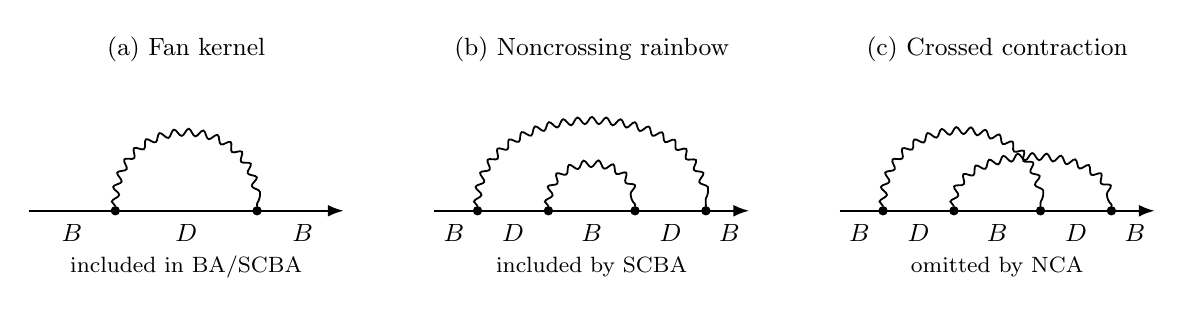
\begin{tikzpicture}[
   x=1cm,y=1cm,
   exciton/.style={line width=0.75pt,-{Latex[length=2mm,width=1.5mm]}},
   phonon/.style={decorate,decoration={snake,amplitude=0.45mm,
     segment length=1.8mm},line width=0.65pt},
   vertex/.style={circle,fill=black,inner sep=1.2pt},
   state/.style={font=\small},
   panel/.style={font=\small}
 ]
  \begin{scope}
   \node[panel] at (2,2.05) {(a) Fan kernel};
   \draw[exciton] (0,0) -- (4,0);
   \node[vertex] at (1.1,0) {};
   \node[vertex] at (2.9,0) {};
   \draw[phonon] (1.1,0.06) .. controls (1.1,1.25) and (2.9,1.25)
     .. (2.9,0.06);
   \node[state] at (0.55,-0.28) {$B$};
   \node[state] at (2.00,-0.28) {$D$};
   \node[state] at (3.48,-0.28) {$B$};
   \node[font=\footnotesize] at (2,-0.72) {included in BA/SCBA};
  \end{scope}
  \begin{scope}[xshift=5.15cm]
   \node[panel] at (2,2.05) {(b) Noncrossing rainbow};
   \draw[exciton] (0,0) -- (4,0);
   \foreach \x in {0.55,1.45,2.55,3.45}{\node[vertex] at (\x,0) {};}
   \draw[phonon] (0.55,0.06) .. controls (0.55,1.45) and (3.45,1.45)
     .. (3.45,0.06);
   \draw[phonon] (1.45,0.06) .. controls (1.45,0.72) and (2.55,0.72)
     .. (2.55,0.06);
   \foreach \x/\s in {0.25/B,1.00/D,2.00/B,3.00/D,3.75/B}
     {\node[state] at (\x,-0.28) {$\s$};}
   \node[font=\footnotesize] at (2,-0.72) {included by SCBA};
  \end{scope}
  \begin{scope}[xshift=10.30cm]
   \node[panel] at (2,2.05) {(c) Crossed contraction};
   \draw[exciton] (0,0) -- (4,0);
   \foreach \x in {0.55,1.45,2.55,3.45}{\node[vertex] at (\x,0) {};}
   \draw[phonon] (0.55,0.06) .. controls (0.55,1.28) and (2.55,1.28)
     .. (2.55,0.06);
   \draw[phonon] (1.45,0.06) .. controls (1.45,0.84) and (3.45,0.84)
     .. (3.45,0.06);
   \foreach \x/\s in {0.25/B,1.00/D,2.00/B,3.00/D,3.75/B}
     {\node[state] at (\x,-0.28) {$\s$};}
   \node[font=\footnotesize] at (2,-0.72) {omitted by NCA};
  \end{scope}
 \end{tikzpicture}
 \caption{Diagrammatic hierarchy of the site-local closure.  Solid arrows are
 dimer exciton propagators and wavy arcs are difference-mode phonon
 contractions.  The leading $B\to D\to B$ Fan channel and its nested
 noncrossing repetitions are retained by SCBA; the first crossed contraction
 is omitted.  Near the positive-$J$ one-phonon resonance its dark-state
 intermediate propagation can be enhanced, but the dominant overall
 limitation remains the $S$-controlled local Franck--Condon combinatorics.
 The diagrams show contraction topology, not a momentum-resolved
 calculation.}
 \label{fig:diagrams}
\end{figure}

ED measures the total closure error.  Parity identifies which exact
bright--dark avoided crossings are allowed, but a Wasserstein cusp alone does
not identify a missing diagram.  In particular, even-control structure can
come from replica alignment, pole-shift sensitivity, common-mode structure,
and the incomplete NCA diagram subset.  An explicit one-crossing/OCA or
vertex-corrected calculation would be required to quantify the contribution
of the lowest crossed diagram to any given cusp.

\subsection{Broadening and metric scope}

The retarded $\eta$ broadens delta peaks; it is not a phonon damping rate and
does not shorten the bath memory.  Broadening can hide resolved discrepancies
but cannot restore crossed contractions or vertex corrections.  The
Wasserstein distance is a robust global transport metric, but it does not by
itself diagnose peak topology or isolate an individual pole error.  The
resonance-sweep spectra and exact parity analysis supply complementary
structural information.

\section{Conclusions}

The primary limitation of site-local SCBA/NCA is the $S$-controlled local
multiphonon combinatorial error already present at $J=0$.  Finite $J$ adds a
secondary commensurability correction, whose cleanest resonant breakdown is
the positive-$J$, odd-parity, emission-accessible conversion at $T=0$.  The
leading Fan $B\to D\to B$ channel is included; near resonance, dark-state
propagation instead amplifies sensitivity to omitted higher-order crossed
contractions and vertex corrections.  Large splitting suppresses difference-mode
conversion but leaves the common-mode Franck--Condon problem, so detuning
alone never guarantees exactness.  The practical rule is hierarchical: small
effective $S$ first, then off-resonant detuning.  This is a crossover
diagnostic, not a universal threshold, and ED alone cannot attribute a cusp
to one crossed diagram.

\end{document}
